\documentclass[a4paper,10pt]{article}

% Encoding and typeface: XeLaTeX with Latin Modern Roman (fontspec default), English via polyglossia
\usepackage{fontspec}
\usepackage{polyglossia}
\setdefaultlanguage[variant=british]{english}

% Layout (tight margins)
\usepackage[a4paper,top=1.2cm,bottom=1.3cm,left=1.3cm,right=1.3cm]{geometry}

% Typography
\usepackage{microtype}
\usepackage{setspace}
\setstretch{0.92}

% Paragraph settings
\setlength{\parindent}{0pt}
\setlength{\parskip}{3pt}

% Section styling
\usepackage{titlesec}
\titleformat{\section}{\bfseries\normalsize}{\thesection.}{0.4em}{}
\titlespacing*{\section}{0pt}{6pt}{3pt}

% Better lists
\usepackage{enumitem}
\setlist{noitemsep, topsep=2pt}

% Mathematics, tables, figures
\usepackage{amsmath}
\usepackage{booktabs}
\usepackage{graphicx}
\usepackage[font=small,labelfont=bf,labelsep=period,skip=3pt]{caption}
\setlength{\textfloatsep}{8pt}
\setlength{\floatsep}{6pt}

\newcommand{\HeThreeMax}{0.5506}
\newcommand{\PhiZeroSixth}{0.0665}
\newcommand{\TThreeConst}{0.1100}
\newcommand{\ExpConst}{0.1330}
\newcommand{\ExpDThirty}{0.0243}
\newcommand{\LapDThirty}{0.00230}
\newcommand{\ExpOverLap}{10.6}
\newcommand{\UniDOne}{0.0572}
\newcommand{\ExpDOne}{0.159}
\newcommand{\UniRatio}{1.000}
\newcommand{\UniNBelow}{3}
\newcommand{\UniNLead}{3}
\newcommand{\UniDTenK}{$2.75\times 10^{-6}$}
\newcommand{\LapRatio}{1.000}
\newcommand{\LapNBelow}{7}
\newcommand{\LapNLead}{7}
\newcommand{\LapDTenK}{$6.88\times 10^{-6}$}
\newcommand{\TFiveRatio}{0.974}
\newcommand{\TFiveNBelow}{8}
\newcommand{\TFiveNLead}{14}
\newcommand{\TFiveDTenK}{$1.34\times 10^{-5}$}
\newcommand{\TThreeRatio}{0.998}
\newcommand{\TThreeNBelow}{116}
\newcommand{\TThreeNLead}{121}
\newcommand{\TThreeDTenK}{0.00110}
\newcommand{\ChiRatio}{1.000}
\newcommand{\ChiNBelow}{71}
\newcommand{\ChiNLead}{71}
\newcommand{\ChiDTenK}{$8.41\times 10^{-4}$}
\newcommand{\ExpRatio}{1.000}
\newcommand{\ExpNBelow}{177}
\newcommand{\ExpNLead}{177}
\newcommand{\ExpDTenK}{0.00133}
\newcommand{\LogNLead}{226}
\newcommand{\FNLead}{662}
\newcommand{\TThreeSqrtD}{0.1097}
\newcommand{\NoiseExact}{0.0193}
\newcommand{\NoiseQ}{0.0303}
\newcommand{\NoiseAsym}{0.0194}
\newcommand{\NoiseGrid}{0.0171}
\newcommand{\VoneNormalTenK}{0.0151}
\newcommand{\VoneUniTenK}{0.0134}
\newcommand{\VoneExpTenK}{0.0173}
\newcommand{\VoneUniTen}{0.0101}
\newcommand{\UniDTen}{0.00281}
\newcommand{\NormalFramesBelow}{30}
\newcommand{\UniFramesBelow}{30}
\newcommand{\LapFramesBelow}{30}
\newcommand{\TFiveFramesBelow}{30}
\newcommand{\ChiFramesBelow}{26}
\newcommand{\ExpFramesBelow}{22}
\newcommand{\ExpNoiseN}{48}
\newcommand{\UniNoiseN}{2}
\newcommand{\ParetoFramesCut}{19}
\newcommand{\ParetoMaxKs}{0.151}
\newcommand{\FFramesCut}{2}
\newcommand{\RUniThirty}{8.8\times 10^{5}}
\newcommand{\RUniThousand}{1.0\times 10^{9}}
\newcommand{\RExpThirty}{1{,}279}
\newcommand{\RExpThousand}{42{,}676}
\newcommand{\RTThreeThousand}{63{,}293}
\newcommand{\IqrSlopeParetoTwoFive}{-0.46}
\newcommand{\IqrSlopeParetoOneFive}{-0.30}
\newcommand{\IqrSlopeCauchy}{-0.006}
\newcommand{\CauchyIqrOne}{1.98}
\newcommand{\CauchyIqrTenK}{2.01}
\newcommand{\ParetoSlope}{-0.23}
\newcommand{\ParetoTen}{0.152}
\newcommand{\ParetoHundred}{0.085}
\newcommand{\ParetoThousand}{0.049}
\newcommand{\ParetoTenK}{0.031}
\newcommand{\LogSlope}{-0.42}
\newcommand{\FSlope}{-0.40}
\newcommand{\LogSimTen}{0.045}
\newcommand{\LogLeadTen}{0.048}
\newcommand{\FSimTen}{0.061}
\newcommand{\FLeadTen}{0.081}
\newcommand{\NoiseHundredK}{0.0027}


\begin{document}

% Header (top-right)
\begin{flushright}
\small \textbf{Compiled on:} \today
\end{flushright}

\vspace{-6pt}
\hrule
\vspace{24pt}

\textbf{TITLE:} How fast does the central limit theorem work? Exact distances, simulation noise and heavy tails

\textbf{SUBJECT:} Aim, method and results of the analyses in version 2 of the \texttt{CLT-speed-race-exercise} repository

\textbf{PREPARED BY:} Muhammed İkbal Yılmaz (myucanlar@gmail.com)

\vspace{12pt}

\section{Aim and scope}

Let $X_1, X_2, \dots$ be independent draws from a distribution with mean $\mu$ and variance $\sigma^2$, and let
$Z_n = \sqrt n\,(\bar X_n - \mu)/\sigma$ be the standardized sample mean, with distribution function $F_n$. If
$0 < \sigma^2 < \infty$, the central limit theorem (CLT) says that $F_n(x) \to \Phi(x)$ for every $x$. How fast this happens is
measured here by the Kolmogorov distance
\[
D_n = \sup_x \lvert F_n(x) - \Phi(x)\rvert ,
\]
the largest error in any probability $P(Z_n \le x)$ computed from the normal approximation. Version 1 of this project animated
simulations of $Z_n$ with $R = 2000$ replications for ten distributions and grouped them by eye: fast (Normal, Uniform), slower
(Exponential, Laplace), very slow (Student-t with few degrees of freedom), and failing (Pareto with tail index $\le 2$, Cauchy).
This note asks three questions:

\begin{enumerate}
  \item \textbf{How large is $D_n$ exactly, and what determines how fast it falls?} Six of the distributions allow an exact
  computation.
  \item \textbf{What can a simulation with $R = 2000$ replications measure?} Even an exactly normal $Z_n$ gives a simulated
  distance above zero.
  \item \textbf{What happens for the remaining distributions:} Lognormal, F and Pareto, which have no exact method here, and
  Cauchy and Pareto with infinite variance, where version 1 stopped?
\end{enumerate}

All distributions use the default parameters of version 1: Uniform(0, 1), Exponential(1), Laplace(0, 1), Lognormal with
$\sigma = 0.6$, Chi-square(5), F(5, 10), Student-t(5), Pareto with tail index 2.5. Student-t(3) is added as the smallest integer
number of degrees of freedom with finite variance.

\section{Method}

\begin{itemize}
  \item \textbf{Exact distances.} For Exponential and Chi-square the sum of $n$ draws is gamma distributed, so $F_n$ is a
  regularized incomplete gamma function. For Uniform with $n \le 40$ the sum has the Irwin--Hall distribution, evaluated in exact
  rational arithmetic. For the other cases (Laplace, Uniform with $n > 40$, Student-t), $F_n - \Phi$ is obtained by inverting the
  difference of the two characteristic functions with the Gil-Pelaez (1951) formula and Gauss--Legendre quadrature. Against the
  exact methods, and against closed forms for Laplace ($n = 2$) and Student-t ($n = 1$), this inversion agrees to within
  $3\times 10^{-15}$. The supremum is located on a grid of step $0.02$ on $[-8, 8]$ and refined numerically.
  \item \textbf{Leading terms.} For a continuous distribution with finite fourth moment, the Edgeworth expansion (Hall, 1992) gives
  $F_n(x) - \Phi(x) = -\varphi(x)\bigl[\tfrac{\gamma}{6\sqrt n}He_2(x) + \tfrac{\kappa_4}{24n}He_3(x) + \tfrac{\gamma^2}{72n}He_5(x)\bigr]
  + o(1/n)$, with skewness $\gamma$, excess kurtosis $\kappa_4$ and Hermite polynomials $He_k$. For $\gamma \ne 0$ the leading term
  of $D_n$ is $\lvert\gamma\rvert\varphi(0)/(6\sqrt n) = \PhiZeroSixth\,\lvert\gamma\rvert/\sqrt n$; for $\gamma = 0$ it is
  $\lvert\kappa_4\rvert \cdot \HeThreeMax/(24n)$, where $\HeThreeMax = \max_x\lvert He_3(x)\varphi(x)\rvert$. Student-t(3) has no finite
  third absolute moment. Its standardized characteristic function is $(1+\lvert s\rvert)e^{-\lvert s\rvert} = 1 - s^2/2 +
  \lvert s\rvert^3/3 + O(s^4)$, and the term $\lvert s\rvert^3/3$ gives the leading term $\TThreeConst/\sqrt n$ (derived for this
  note and computed numerically).
  \item \textbf{Simulation.} The simulation of version 1 is repeated draw for draw (same seed, same calls of the random number
  generator); it reproduces four distances printed in the frames that version 1 saved. The noise of a simulation is measured
  by the Kolmogorov statistic of $R$ draws from the true distribution, whose exact distribution is available in SciPy
  (\texttt{scipy.stats.kstwo}).
  \item \textbf{Checks.} Seventeen unit tests compare the code with independent computations: moments with SciPy, characteristic
  functions with numerical Fourier integrals of the densities, the inversion with exact distribution functions, the supremum
  with a brute-force search.
\end{itemize}

\section{Analysis 1: The exact speed of convergence (Figure~\ref{fig:exact}, Table~\ref{tab:summary})}

\textbf{Why.} A ranking of distributions by eye cannot say how much faster one converges than another, or why. The exact $D_n$
answers the first question, and the comparison with the leading terms answers the second.

\textbf{Method.} $D_n$ for 41 values of $n$ from 1 to $10^4$, evenly spaced on a log scale, for six distributions. For each, the
smallest $n$ with $D_n < 0.01$, found by computing $D_n$ for every $n$ up to that point and checking the following 200 values.

\textbf{How to read the figure.} Left: both axes are logarithmic, so a distance proportional to $n^{-1/2}$ is a line of slope
$-1/2$, and one proportional to $n^{-1}$ a line of slope $-1$. Dashed lines are the leading terms. Right: the ratio of $D_n$ to its
leading term; a curve that approaches 1 means that the leading term explains the speed of convergence.

\begin{figure}[h]
\centering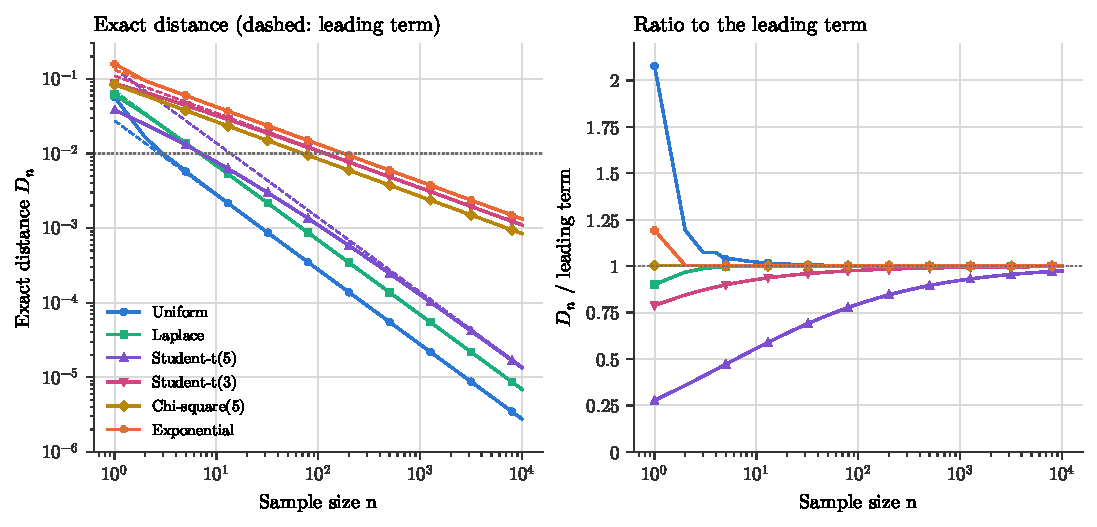
\includegraphics[width=0.9\linewidth]{../figures/fig1_exact_speed.pdf}
\caption{Exact Kolmogorov distance between the standardized mean and the normal distribution. Left: $D_n$ (solid) and its
leading term (dashed); dotted: $0.01$. Right: $D_n$ divided by its leading term.}\label{fig:exact}
\end{figure}

\begin{table}[h]
\centering\footnotesize
\caption{Skewness $\gamma$, excess kurtosis $\kappa_4$, leading term of $D_n$, exact $D_n$, and the smallest $n$ with
$D_n < 0.01$, exact and as predicted by the leading term. --: does not exist, or no exact method here.}\label{tab:summary}
\begin{tabular}{lrrrrrrr}
\toprule
Distribution & $\gamma$ & $\kappa_4$ & Leading term & $D_{30}$ & $D_{1000}$ & $n$ for $D_n<0.01$ & by leading term \\
\midrule
Normal & 0 & $0$ & 0 & 0 & 0 & 1 & -- \\
Uniform & 0 & $-1.20$ & $0.0275\,n^{-1}$ & $9.24\times 10^{-4}$ & $2.75\times 10^{-5}$ & 3 & 3 \\
Laplace & 0 & $3.00$ & $0.0688\,n^{-1}$ & 0.00230 & $6.88\times 10^{-5}$ & 7 & 7 \\
Student-t(5) & 0 & $6.00$ & $0.1376\,n^{-1}$ & 0.00314 & $1.27\times 10^{-4}$ & 8 & 14 \\
Student-t(3) & -- & -- & $0.1100\,n^{-1/2}$ & 0.0192 & 0.00345 & 116 & 121 \\
Chi-square(5) & 1.26 & $2.40$ & $0.0841\,n^{-1/2}$ & 0.0154 & 0.00266 & 71 & 71 \\
Exponential & 2.00 & $6.00$ & $0.1330\,n^{-1/2}$ & 0.0243 & 0.00421 & 177 & 177 \\
Lognormal(0.6) & 2.26 & $10.3$ & $0.1503\,n^{-1/2}$ & -- & -- & -- & 226 \\
F(5, 10) & 3.87 & $50.9$ & $0.2571\,n^{-1/2}$ & -- & -- & -- & 662 \\
Pareto(2.5) & -- & -- & -- & -- & -- & -- & -- \\
Cauchy & \multicolumn{7}{l}{no mean or variance} \\
\bottomrule

\end{tabular}
\end{table}

\textbf{Finding.} The distributions fall into two groups. For the symmetric distributions with a finite fourth moment (Uniform,
Laplace, Student-t(5)) $D_n$ falls like $1/n$; for the skewed ones (Chi-square(5), Exponential) only like $1/\sqrt n$. Student-t(3)
is symmetric but also falls like $1/\sqrt n$. At $n = 10^4$ the ratio to the leading term is \UniRatio{} (Uniform), \LapRatio{}
(Laplace), \ChiRatio{} (Chi-square), \ExpRatio{} (Exponential) and \TThreeRatio{} (Student-t(3)); for Student-t(5) it approaches 1
more slowly (\TFiveRatio{}). The leading term predicts the smallest $n$ with $D_n < 0.01$ exactly for Uniform, Laplace,
Chi-square and Exponential ($n = \UniNBelow$, $\LapNBelow$, $\ChiNBelow$, $\ExpNBelow$). For Lognormal(0.6) and F(5, 10) it predicts
$n \approx \LogNLead$ and $\FNLead$. At $n = 30$, Exponential is still at $D_{30} = \ExpDThirty$, \ExpOverLap{} times Laplace
($\LapDThirty$).

\textbf{Interpretation.} The speed of convergence is set mainly by the skewness: it decides whether the error falls like $1/\sqrt n$ or
like $1/n$. Heavier tails as such, as long as the fourth moment is finite, do not change the rate: Laplace has heavier tails than the uniform
distribution and converges at the same rate, and version 1 placed it wrongly next to Exponential. What slows Student-t(3) is the infinite third absolute moment, which adds
a $1/\sqrt n$ term without any skewness; Student-t(5), the default of version 1, is already at $D_n < 0.01$ for $n = \TFiveNBelow$.
A single rule such as ``$n \ge 30$'' cannot describe this: among the distributions of version 1 the $n$ needed for $D_n < 0.01$
ranges from $\UniNBelow$ (Uniform) to about $\FNLead$ (F(5, 10), leading-term estimate), and Pareto(2.5) has not reached it at
$n = 10^4$ (analysis 3).

\section{Analysis 2: What a simulation with 2000 replications measures (Figure~\ref{fig:mc})}

\textbf{Why.} Version 1 measured the distance from $R = 2000$ simulated values of $Z_n$, as $\max\lvert\hat F(x) - \Phi(x)\rvert$
over 401 grid points on $[-12, 12]$. With finite $R$, $\hat F$ differs from $F_n$ even when $F_n = \Phi$. The simulated distance can
show convergence only while $D_n$ is above this noise.

\textbf{Method.} The simulation of version 1 for Normal, Uniform and Exponential (seed 42, 30 sample sizes from 10 to $10^4$),
compared with the exact $D_n$. The mean noise for $R = 2000$ is \NoiseExact{} for the exact empirical distance
(95\% quantile \NoiseQ{}; the asymptotic value $\sqrt{\pi/2}\,\ln 2/\sqrt R$ is \NoiseAsym{}) and \NoiseGrid{} for the grid distance of
version 1 (400 simulated samples). Right panel: the number of replications at which the mean noise, $0.8687/\sqrt R$, equals $D_n$.

\textbf{How to read the figure.} Left: markers are the distances of version 1, lines the exact $D_n$; the shaded region lies below
the mean noise. Right: the dotted lines mark the default and the largest $R$ that version 1 offered.

\begin{figure}[h]
\centering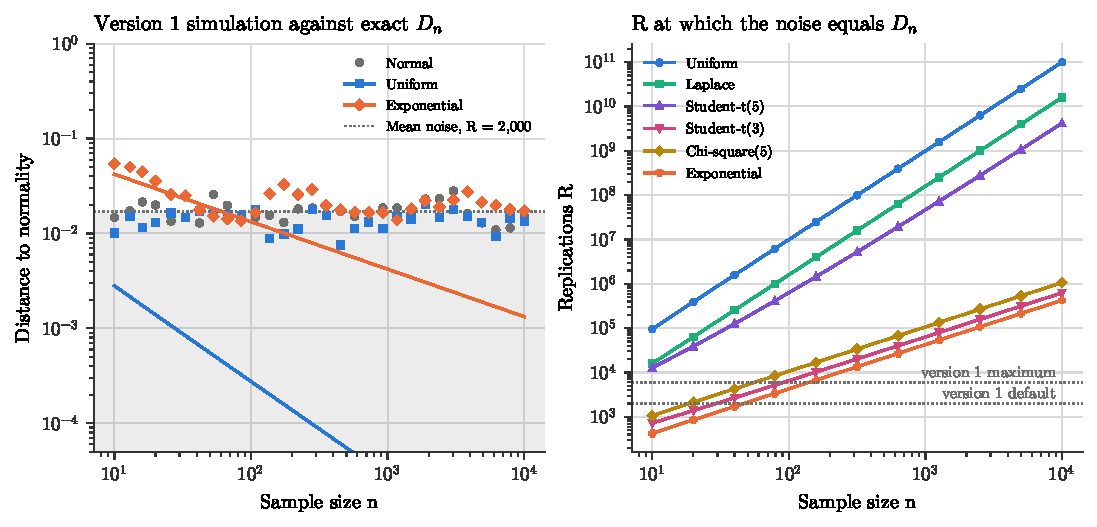
\includegraphics[width=0.9\linewidth]{../figures/fig2_monte_carlo.pdf}
\caption{Left: simulated distances of version 1 (markers; $R = 2000$, seed 42) and exact $D_n$ (lines); dotted: mean noise of the grid
distance of version 1. Right: replications needed for the mean noise to equal $D_n$.}\label{fig:mc}
\end{figure}

\textbf{Finding.} For the Normal distribution $Z_n$ is exactly normal, yet version 1 reports \VoneNormalTenK{} at $n = 10^4$; for
Uniform it reports \VoneUniTenK{}, while the exact distance is \UniDTenK{}. The exact distance falls below the mean noise of the exact empirical distance
(\NoiseExact{}) from $n = \ExpNoiseN$ for Exponential and from $n = \UniNoiseN$ for Uniform. Of the 30 frames of each run, the exact distance was below the noise of version 1 in \UniFramesBelow{}
for Uniform, Laplace and Student-t(5), in \ChiFramesBelow{} for Chi-square(5) and in \ExpFramesBelow{} for Exponential. To make the
mean noise as small as $D_n$, Uniform needs $R \approx \RUniThirty$ replications at $n = 30$ and $\RUniThousand$ at $n = 1000$;
Exponential needs $\RExpThirty$ and $\RExpThousand$. Version 1 also drew the difference $\hat F - \Phi$ with fixed limits of about
$\pm 0.055$; for Pareto(2.5) the distance exceeded them in \ParetoFramesCut{} of 30 frames (up to \ParetoMaxKs{}).

\textbf{Interpretation.} Most frames of the race of version 1 show simulation noise, not convergence: from a few dozen draws on,
every distribution of the race except Pareto(2.5) looks equally close to normal. A simulation can only resolve distances larger than about
$0.87/\sqrt R$, so differences between symmetric distributions at moderate $n$ would need millions to billions of replications. Exact
computation is the only practical way to compare them.

\section{Analysis 3: Heavy tails (Figure~\ref{fig:heavy})}

\textbf{Why.} Two questions are left from version 1: how fast Lognormal, F and Pareto(2.5) converge, which have no exact method
here, and what the sample mean does when the variance is infinite, where version 1 only printed a message.

\textbf{Method.} (a) Interquartile range (IQR) of $\bar X_n$, which exists even without a finite variance: Pareto with tail indices
2.5 and 1.5 and Cauchy, $n$ from 1 to $10^4$, $R = 20{,}000$ paths ($100{,}000$ for Pareto(2.5)); for comparison the exact IQR
$2 \cdot 0.6745/\sqrt n$ of Normal(0, 1). (b) The simulated distance of $Z_n$ for Lognormal(0.6), F(5, 10) and Pareto(2.5) with
$R = 100{,}000$ paths (mean noise \NoiseHundredK{}). Slopes are fitted on the log--log scale for $n \ge 10$ where the simulated
distance exceeds three times the noise.

\textbf{How to read the figure.} Both panels are logarithmic. Left: a slope of $-1/2$ is the $1/\sqrt n$ shrinking of the CLT; a flat
line means that averaging does not reduce the spread. Right: dashed lines are the leading terms where the skewness exists.

\begin{figure}[h]
\centering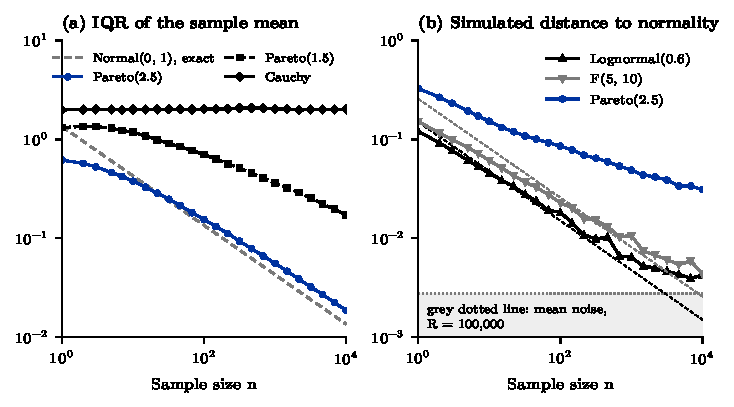
\includegraphics[width=0.9\linewidth]{../figures/fig3_heavy_tails.pdf}
\caption{Left: IQR of the sample mean. Right: simulated distance of $Z_n$ to the normal distribution ($R = 100{,}000$), with leading
terms (dashed); shaded: below the mean noise.}\label{fig:heavy}
\end{figure}

\textbf{Finding.} The IQR of the Cauchy mean is \CauchyIqrOne{} at $n = 1$ and \CauchyIqrTenK{} at $n = 10^4$ (slope
$\IqrSlopeCauchy$): the mean of $n$ Cauchy variables has the same Cauchy distribution as one of them. For Pareto(1.5), which has a
mean but no variance, the slope for $n \ge 100$ is $\IqrSlopeParetoOneFive$, close to $1/\alpha - 1 = -1/3$ from the generalized
CLT (Gnedenko and Kolmogorov, 1954); for Pareto(2.5) it is $\IqrSlopeParetoTwoFive$, still approaching $-1/2$. For Lognormal(0.6) and
F(5, 10) the simulated distance falls with slopes $\LogSlope$ and $\FSlope$; at $n = 10$ it is \LogSimTen{} against a leading term
of \LogLeadTen{} (Lognormal) and \FSimTen{} against \FLeadTen{} (F). Pareto(2.5), whose third moment is infinite, converges much more
slowly: \ParetoTen{}, \ParetoHundred{}, \ParetoThousand{} and \ParetoTenK{} at $n = 10$, $10^2$, $10^3$, $10^4$ (slope
$\ParetoSlope$). At $n = 10^4$ it is further from normal than Exponential at $n = 30$.

\textbf{Interpretation.} With infinite variance the spread of the sample mean does not shrink like $1/\sqrt n$. For Cauchy averaging
does not reduce it at all. For Pareto(1.5) the mean still converges to $\mu$, but at the rate $n^{1/\alpha - 1}$ and with a non-normal
(stable) limit, so a histogram standardized with $\sqrt n$ cannot settle. Finite variance alone guarantees convergence but not its
speed. The Lyapunov--Katz bound (Katz, 1963) states $D_n \le C\,\nu_{2+\delta}\, n^{-\delta/2}$, $0 < \delta \le 1$, where
$\nu_{2+\delta} = E\lvert Y\rvert^{2+\delta}$ for the standardized variable $Y$. For Pareto(2.5) only moments of order below 2.5 exist, so
the bound applies only with $\delta < 0.5$ and guarantees a decrease only at a rate of up to about $n^{-1/4}$. The measured slope,
$\ParetoSlope$, is of this order.

\section{Conclusions and limitations}

\begin{itemize}
  \item The speed of convergence is governed mainly by the skewness: $D_n$ falls like $1/n$ for symmetric distributions with a finite
  fourth moment and like $1/\sqrt n$ for skewed ones, with the constant given by the leading term of the Edgeworth expansion.
  Infinite third moments (Student-t(3), Pareto(2.5)) slow convergence further.
  \item A simulation with $R$ replications cannot resolve distances below about $0.87/\sqrt R$. Most frames of the race of version 1
  show this noise.
  \item With infinite variance the CLT in its usual form does not apply: the Cauchy mean does not concentrate, and the Pareto(1.5)
  mean concentrates like $n^{-1/3}$.
  \item The Kolmogorov distance measures the largest error in a probability, not the relative error in the tails, which can be much
  larger. Lognormal, F and Pareto are studied by simulation only. Only the default parameters of version 1 are used.
\end{itemize}

\section*{References}
{\small
Gil-Pelaez, J. (1951). Note on the inversion theorem. \textit{Biometrika}, 38(3--4), 481--482.\\
Gnedenko, B. V., Kolmogorov, A. N. (1954). \textit{Limit Distributions for Sums of Independent Random Variables}. Addison-Wesley.\\
Hall, P. (1992). \textit{The Bootstrap and Edgeworth Expansion}. Springer.\\
Katz, M. L. (1963). Note on the Berry--Esseen theorem. \textit{Annals of Mathematical Statistics}, 34(3), 1107--1108.\\
SciPy documentation: \texttt{scipy.special.gammainc}, \texttt{scipy.stats.kstwo}.

\smallskip
An AI coding assistant was used in writing the code and in preparing this note. All numbers are generated from
\texttt{figures/*.csv} by \texttt{make\_paper.py}.
}

\end{document}
